\documentclass[10pt, a4paper]{article}

\usepackage[utf8]{inputenc}
\usepackage[english,spanish]{babel}
\usepackage[left=25mm, right=25mm, top=35mm, bottom=30mm, headheight=35mm]{geometry}
\usepackage{graphicx}
\usepackage{xcolor}
\usepackage{fancyhdr}
\usepackage{hyperref}
\usepackage{setspace}
\usepackage{float}
\usepackage{listings}
\lstset{
  basicstyle=\ttfamily,
  keywordstyle=\color{blue},
  commentstyle=\color{green},
  stringstyle=\color{red},
  showstringspaces=false,
  breaklines=true,
  frame=single,
  backgroundcolor=\color{lightgray},
  columns=fullflexible
}
\lstdefinestyle{JavaStyle}{
    language=Java,
    basicstyle=\small\ttfamily,
    keywordstyle=\color{blue},
    commentstyle=\color{green},
    stringstyle=\color{purple},
    tabsize=4,
    showspaces=false,
    showstringspaces=false
} 
\lstdefinestyle{JavaScriptStyle}{
    language=JavaScript,
    basicstyle=\small\ttfamily,
    keywordstyle=\color{blue},
    commentstyle=\color{green},
    stringstyle=\color{purple},
    tabsize=4,
    showspaces=false,
    showstringspaces=false
} 

% Define background color
\definecolor{background}{HTML}{2E3440}

% Syntax customization
\usepackage{minted}
\usemintedstyle{nord}
\setminted{bgcolor=background}
\setminted{breaklines}

% Variables
\newcommand{\university}{Universidad Nacional de San Agustín de Arequipa}
\newcommand{\faculty}{Facultad de Ingeniería de Producción y Servicios}
\newcommand{\program}{Escuela Profesional de Ingeniería de Sistemas}
\newcommand{\semester}{2024 - A}
\newcommand{\course}{img/web_programming}
\newcommand{\topic}{img/Python.png} 
\newcommand{\professor}{Carlo Jose Luis Corrales Delgado}
\newcommand{\students}{Mamani Anahua, Victor Narciso} 
\newcommand{\github}{https://github.com/VictorMA18/Lab05-Python}
\newcommand{\video}{https://drive.google.com/file/d/1EeI8JwQNJr45i3DRMdqxW7Pbtwjt82PL/view}
\newcommand{\mydate}{7 de mayo, 2024}

% Just parts and chapters numbered
\setcounter{secnumdepth}{0}

% Head and foot customization
\pagestyle{fancy}
\lhead{\raisebox{-0.2\height}{
\includegraphics[width=4cm]{img/logo_unsa.png}}}
\chead{\fontsize{8}{8}\selectfont \university \\ \faculty \\ \textbf{\program}}
\rhead{\raisebox{-0.2\height}{
\includegraphics[width=3.5cm]{img/logo_episunsa.png}}}
% \lfoot{Estudiante \student}
\lfoot{Semestre \semester}
\cfoot{}
\rfoot{Pág. \thepage}

\begin{document}

\begin{titlepage}
	\centering
	\includegraphics[width=14cm]{\course} \par
  \vfill \vfill
	\includegraphics[width=15cm]{\topic}\par
  \vfill \vfill
  {\textbf{Profesor(a):} \par}
	\professor \vfill
  {\textbf{Estudiantes:} \par}
	\students \vfill
  {\textbf{Repositorio GitHub:} \par}
  \href{\github}{\github} \vfill
  {\textbf{Video:} \par}
  \href{\video}{\video} \vfill
	{\large \mydate \par}
\end{titlepage}

\section{Ejercicios de Python}
Para iniciar los ejercicios vamos a primero instalar un paquete de python el cual es 
\begin{lstlisting}[language=bash]
  pip install pygame
\end{lstlisting} 

\section{Funciones Picture}
La clase Picture permite realizar diversas operaciones sobre imágenes representadas como listas de cadenas de caracteres. Incluye métodos para crear espejos verticales (verticalMirror) y horizontales (horizontalMirror), invertir los colores de la imagen (negative), unir imágenes horizontalmente (join) y verticalmente (up), superponer una imagen sobre otra (under), repetir la imagen horizontalmente (horizontalRepeat) y verticalmente (verticalRepeat), y rotar la imagen 90 grados (rotate). Además, tiene métodos para inicializar una imagen (init), comparar dos imágenes (eq), y una función auxiliar para invertir colores (invColor). Cada método devuelve una nueva instancia de Picture con la transformación aplicada, permitiendo una manipulación flexible de las imágenes
\singlespacing
Para iniciar con los ejercicios tenemos que primero implementar las Funciones de la clase Picture para su posterior uso con funciones para sus objetos
\section{Funciones Picture}  
\begin{figure}[H]
  \centering
  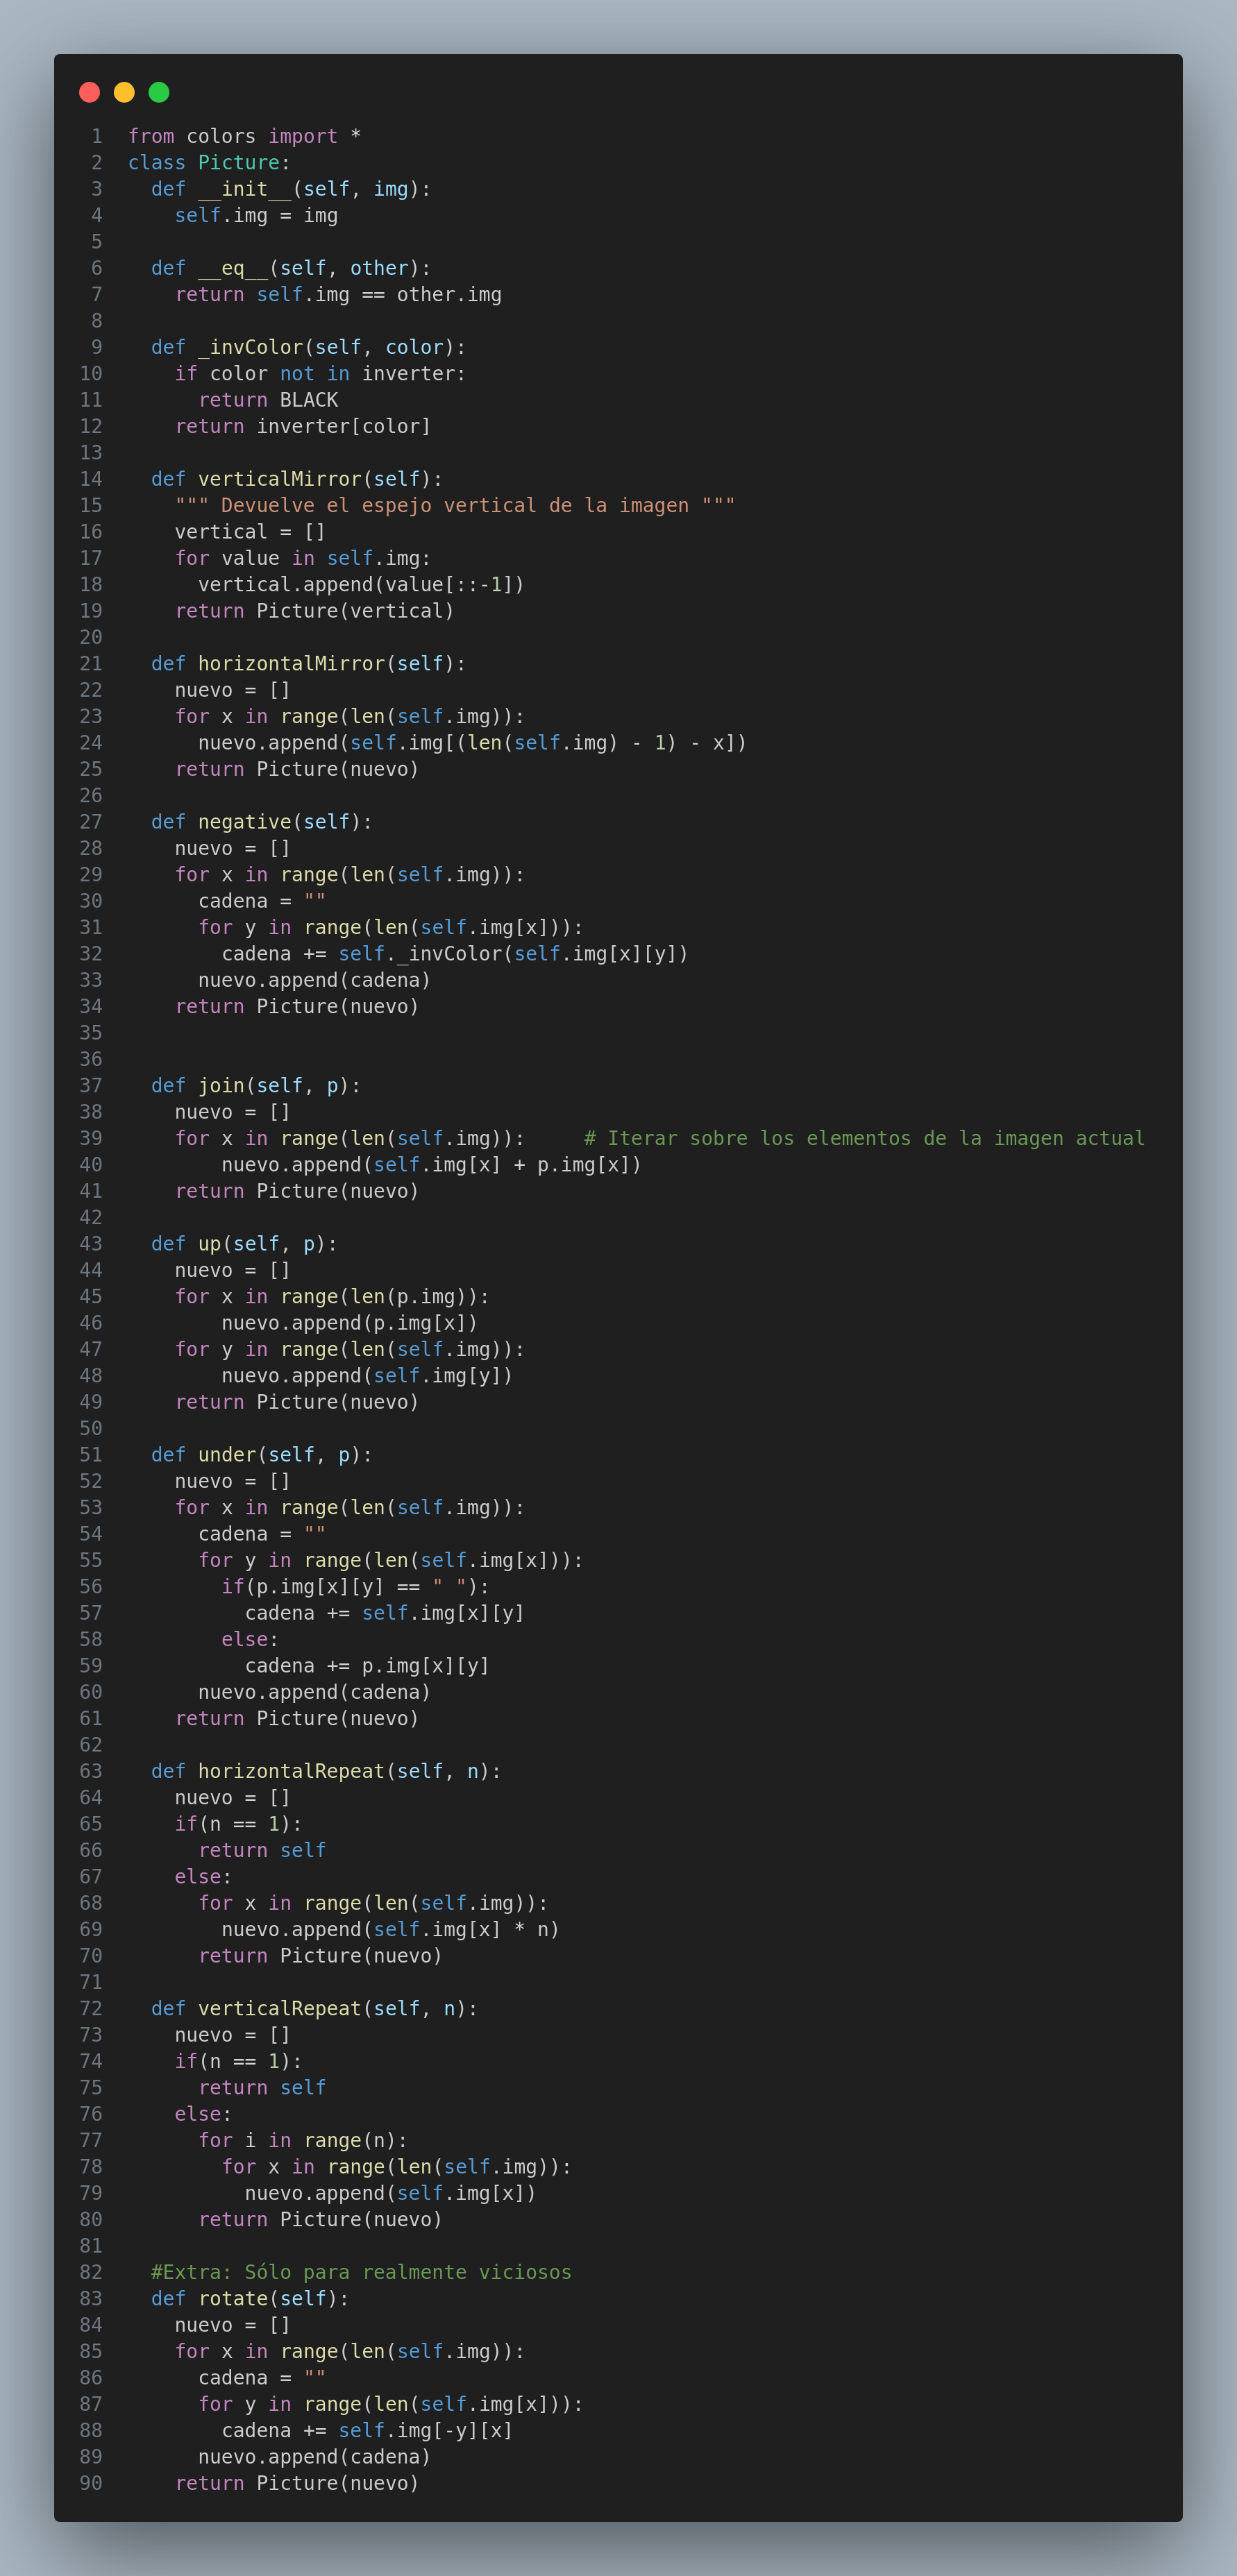
\includegraphics[width=0.7\textwidth]{img/Picture.png}
  \caption{Codigo}
\end{figure}


\section{Primer Ejercicio}
En este código de Python, primero inicializo Pygame y luego importo módulos personalizados para manipular imágenes de piezas de ajedrez. Creo una imagen de un caballo blanco y otra de un caballo negro, que es la versión negativa del blanco. Luego, en un bucle que se ejecuta dos veces, combino estas imágenes de diferentes maneras: si el índice es par, uno el caballo blanco con el negro horizontalmente; si es impar, coloco el caballo blanco sobre su versión negativa. Finalmente, dibujo la imagen resultante usando la función draw, creando así una composición gráfica de caballos blancos y negros según las operaciones realizadas en el bucle.
\singlespacing
Para esto vamos poner el primer codigo python el cual es: 
\begin{figure}[H]
  \centering
  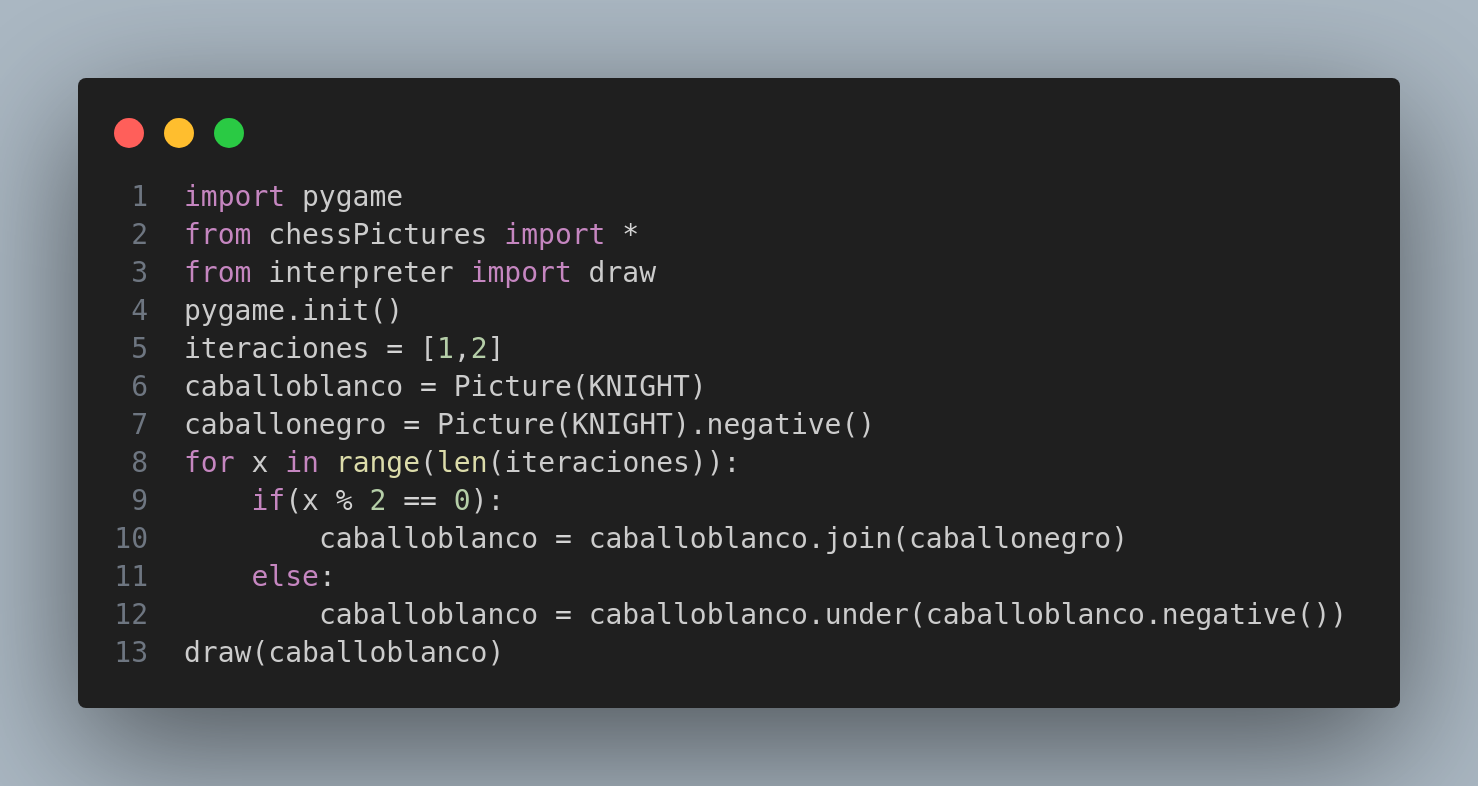
\includegraphics[width=0.7\textwidth]{img/Ej1.png}
  \caption{Codigo}
\end{figure}

\begin{figure}[H]
  \centering
  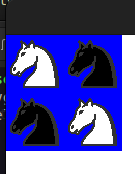
\includegraphics[width=0.7\textwidth]{img/Ejercicio1.png}
  \caption{Ejecucion}
\end{figure}

\section{Segundo Ejercicio}
En este código de Python, primero inicializo Pygame e importo módulos personalizados para manipular imágenes de piezas de ajedrez. Creo una imagen de un caballo blanco y otra de un caballo negro, que es la versión negativa del blanco. Luego, en un bucle que se ejecuta dos veces, combino estas imágenes de diferentes maneras: si el índice es par, uno el caballo blanco con el negro horizontalmente; si es impar, coloco el caballo blanco sobre su versión reflejada verticalmente. Finalmente, dibujo la imagen resultante usando la función draw, creando así una composición gráfica de caballos blancos y negros según las operaciones realizadas en el bucle.
\singlespacing
Para esto vamos poner el segundo codigo python el cual es:  
\begin{figure}[H]
  \centering
  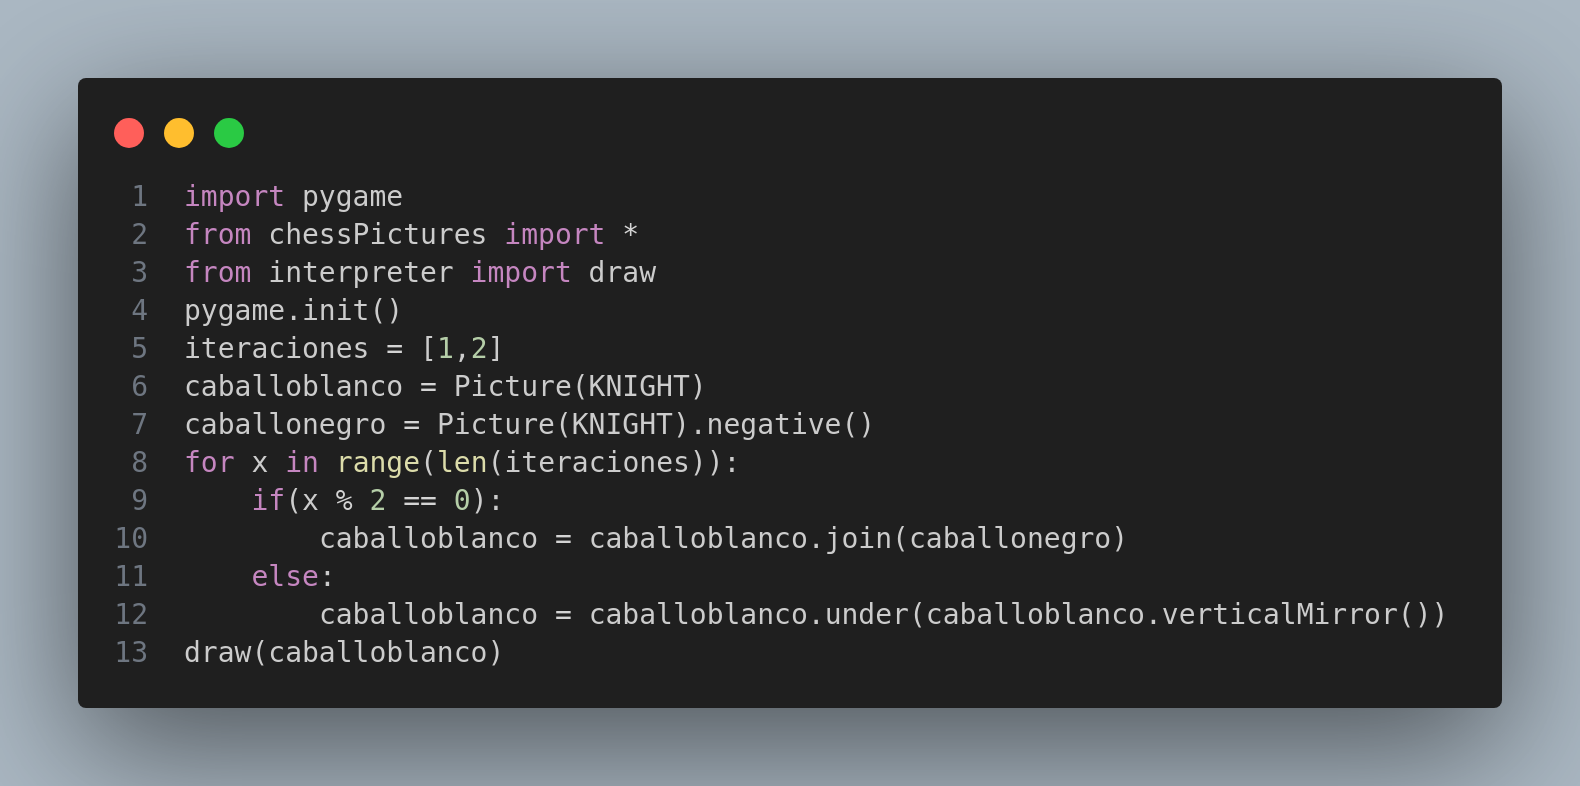
\includegraphics[width=0.7\textwidth]{img/Ej2.png}
  \caption{Codigo}
\end{figure}

\begin{figure}[H]
  \centering
  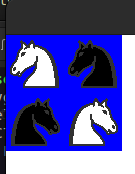
\includegraphics[width=0.7\textwidth]{img/Ejercicio2.png}
  \caption{Ejecucion}
\end{figure}

\section{Tercer Ejercicio}
En este código de Python, primero inicializo Pygame e importo módulos personalizados para trabajar con imágenes de piezas de ajedrez. Creo una imagen de una reina blanca y una imagen vacía. Luego, en un bucle que se ejecuta cinco veces, combino estas imágenes de diferentes maneras: en la primera iteración, coloco la reina blanca sobre la imagen vacía; en las iteraciones posteriores a la segunda, uno la imagen vacía con la reina blanca horizontalmente. Finalmente, dibujo la imagen resultante usando la función draw, creando así una composición gráfica de la reina blanca según las operaciones realizadas en el bucle.
\singlespacing
Para esto vamos poner el tercer codigo python el cual es:  
\begin{figure}[H]
  \centering
  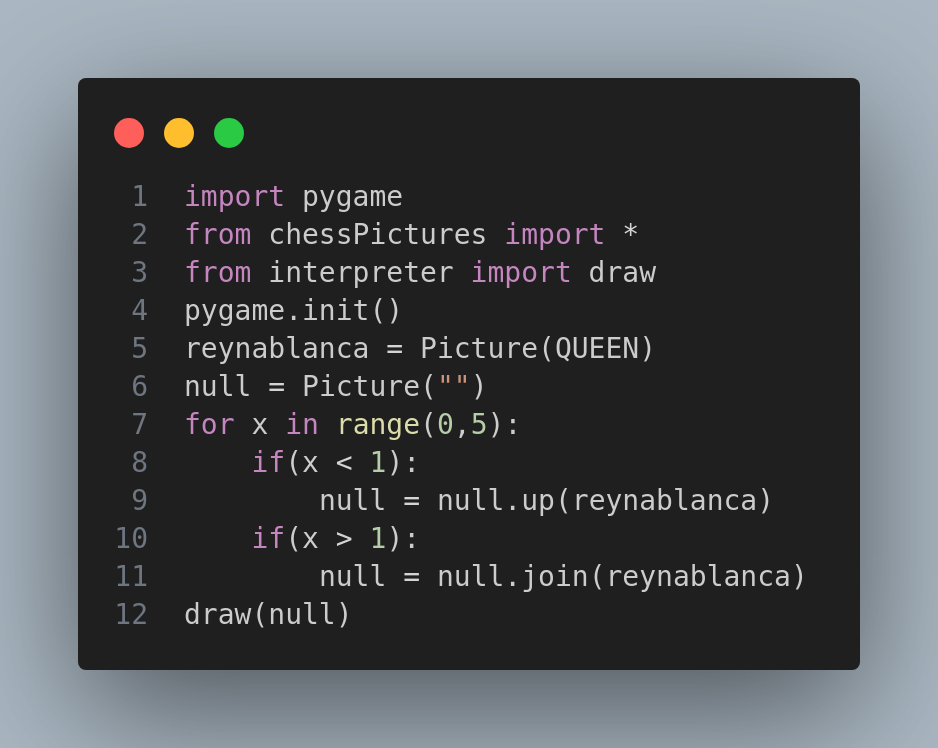
\includegraphics[width=0.7\textwidth]{img/Ej3.png}
  \caption{Codigo}
\end{figure}

\begin{figure}[H]
  \centering
  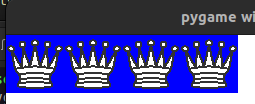
\includegraphics[width=0.7\textwidth]{img/Ejercicio3.png}
  \caption{Ejecucion}
\end{figure}

\section{Cuarto Ejercicio}
En este código de Python, primero inicializo Pygame e importo módulos personalizados para trabajar con imágenes de piezas de ajedrez. Creo imágenes para representar una fila de casillas blancas y negras, así como una imagen vacía. Luego, en un bucle que se ejecuta cuatro veces, combino estas imágenes de diferentes maneras: en la primera iteración, coloco la fila de casillas blancas y negras sobre la imagen vacía; en las iteraciones posteriores, uno la imagen vacía con la fila de casillas blancas y negras horizontalmente. Finalmente, dibujo la imagen resultante usando la función draw, creando así una composición gráfica de casillas blancas y negras según las operaciones realizadas en el bucle.
\singlespacing
Para esto vamos poner el cuarto codigo python el cual es:  
\begin{figure}[H]
  \centering
  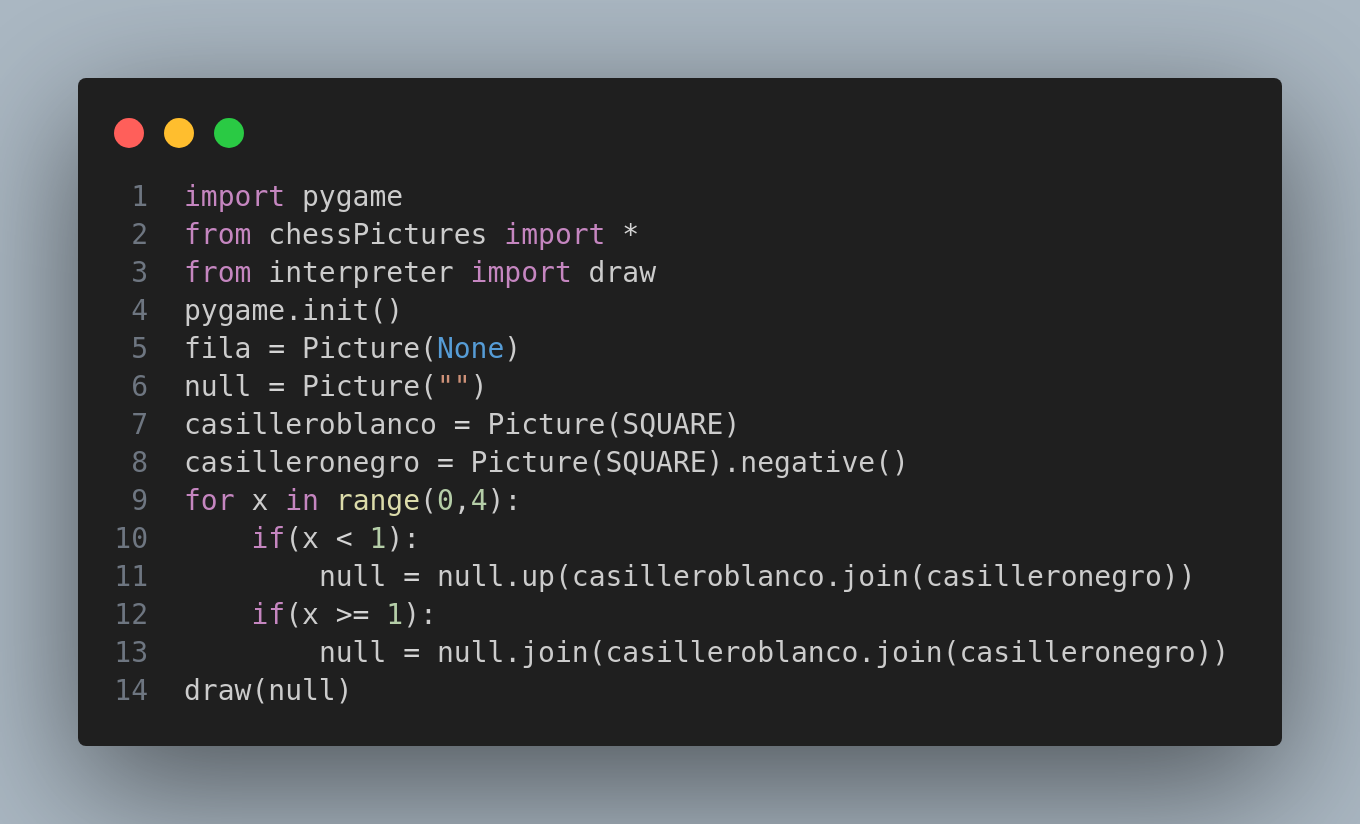
\includegraphics[width=0.7\textwidth]{img/Ej4.png}
  \caption{Codigo}
\end{figure}

\begin{figure}[H]
  \centering
  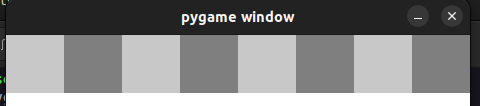
\includegraphics[width=0.7\textwidth]{img/Ejercicio4.png}
  \caption{Ejecucion}
\end{figure}

\section{Quinto Ejercicio}
En este código de Python, primero inicializo Pygame e importo módulos personalizados para trabajar con imágenes de piezas de ajedrez. Creo imágenes para representar una fila de casillas blancas y negras, así como una imagen vacía. Luego, en un bucle que se ejecuta cuatro veces, combino estas imágenes de diferentes maneras: en la primera iteración, coloco la fila de casillas blancas y negras (invertidas) sobre la imagen vacía; en las iteraciones posteriores, uno la imagen vacía con la fila de casillas blancas y negras (invertidas) horizontalmente. Finalmente, dibujo la imagen resultante usando la función draw, creando así una composición gráfica de casillas blancas y negras (invertidas) según las operaciones realizadas en el bucle.
\singlespacing
Para esto vamos poner el quinto codigo python el cual es:  
\begin{figure}[H]
  \centering
  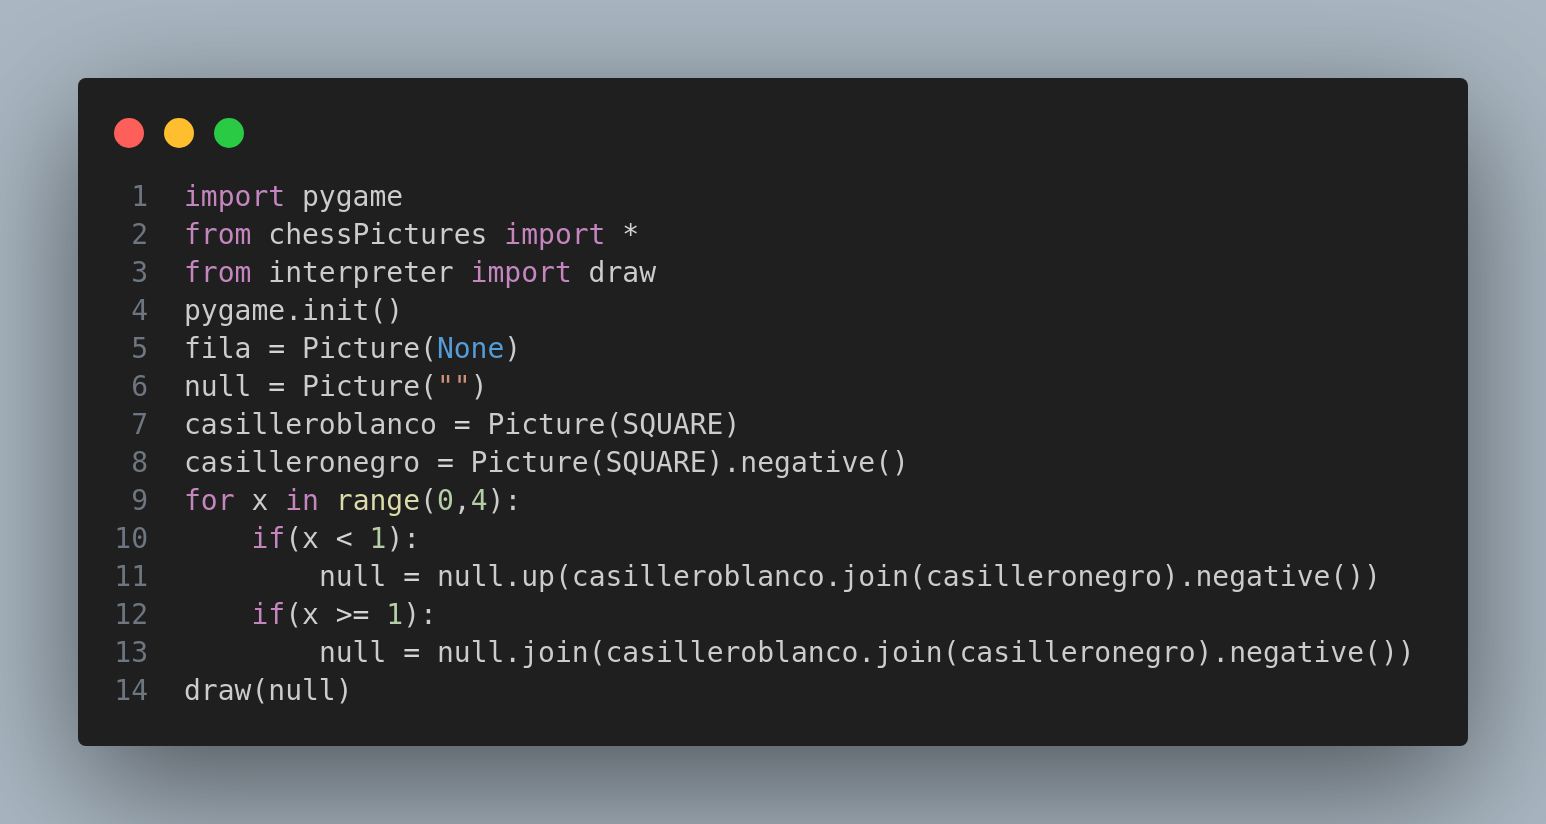
\includegraphics[width=0.7\textwidth]{img/Ej5.png}
  \caption{Codigo}
\end{figure}

\begin{figure}[H]
  \centering
  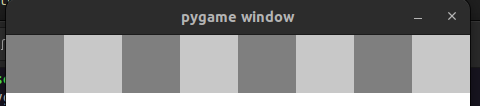
\includegraphics[width=0.7\textwidth]{img/Ejercicio5.png}
  \caption{Ejecucion}
\end{figure}

\section{Sexto Ejercicio}
En este código de Python, primero se inicializa Pygame y se importan módulos personalizados para trabajar con imágenes de piezas de ajedrez. Se crea una imagen vacía y dos imágenes para representar casillas blancas y negras, esta última con un efecto negativo aplicado. Luego, en un bucle que se ejecuta cuatro veces, se combinan estas imágenes para formar una fila de casillas blancas y negras. Después, en otro bucle que se ejecuta dos veces, se aplican operaciones a la imagen resultante: en las iteraciones pares, se coloca la imagen negativa sobre sí misma; en las impares, se coloca la imagen original sobre sí misma. Finalmente, se dibuja la imagen resultante utilizando la función draw, creando así una composición gráfica de casillas blancas y negras con efectos según las operaciones realizadas en los bucles.
\singlespacing
Para esto vamos poner el sexto codigo python el cual es:  
\begin{figure}[H]
  \centering
  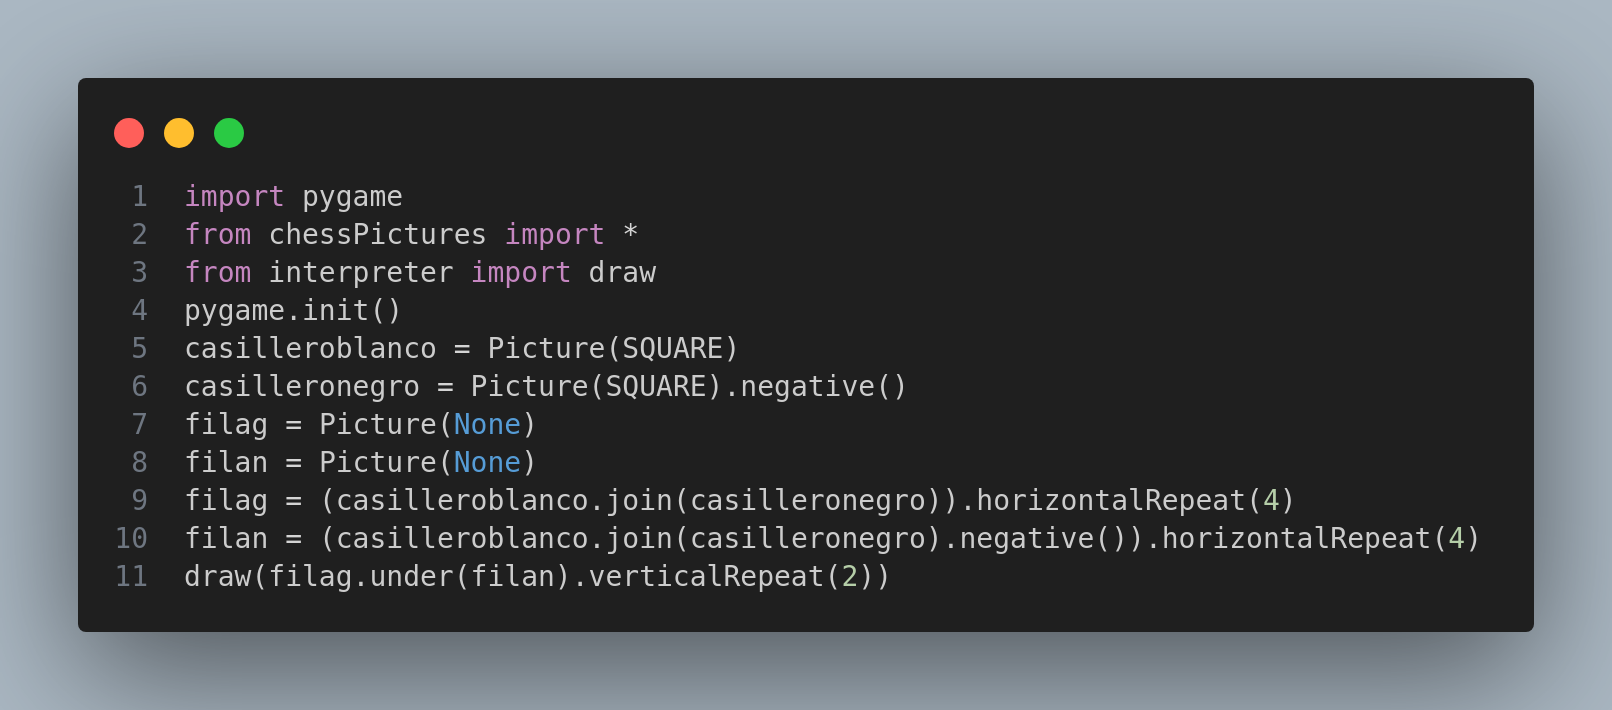
\includegraphics[width=0.7\textwidth]{img/Ej6.png}
  \caption{Codigo}
\end{figure}

\begin{figure}[H]
  \centering
  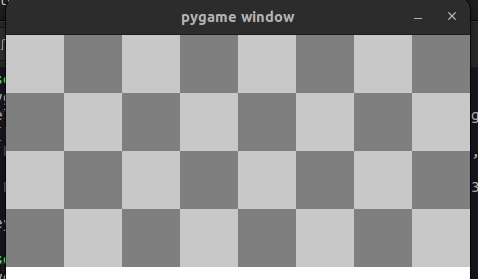
\includegraphics[width=0.7\textwidth]{img/Ejercicio6.png}
  \caption{Ejecucion}
\end{figure}

\section{Septimo Ejercicio}
Este código en Python utiliza Pygame y módulos personalizados para construir un tablero de ajedrez visualmente representado con las piezas correctamente posicionadas. Comienza inicializando Pygame y estableciendo los objetos necesarios para el tablero y las piezas. Luego, mediante bucles y operaciones de unión y superposición, se construyen las diferentes partes del tablero y se colocan las piezas según las reglas del ajedrez. Las piezas se posicionan en la base del tablero, con una fila de peones en la parte inferior y las piezas principales en la parte superior. El resultado es una representación gráfica detallada de un tablero de ajedrez con todas las piezas colocadas correctamente, listo para ser visualizado con la función draw.
\singlespacing
Para esto vamos poner el septimo codigo python el cual es:  
\begin{figure}[H]
  \centering
  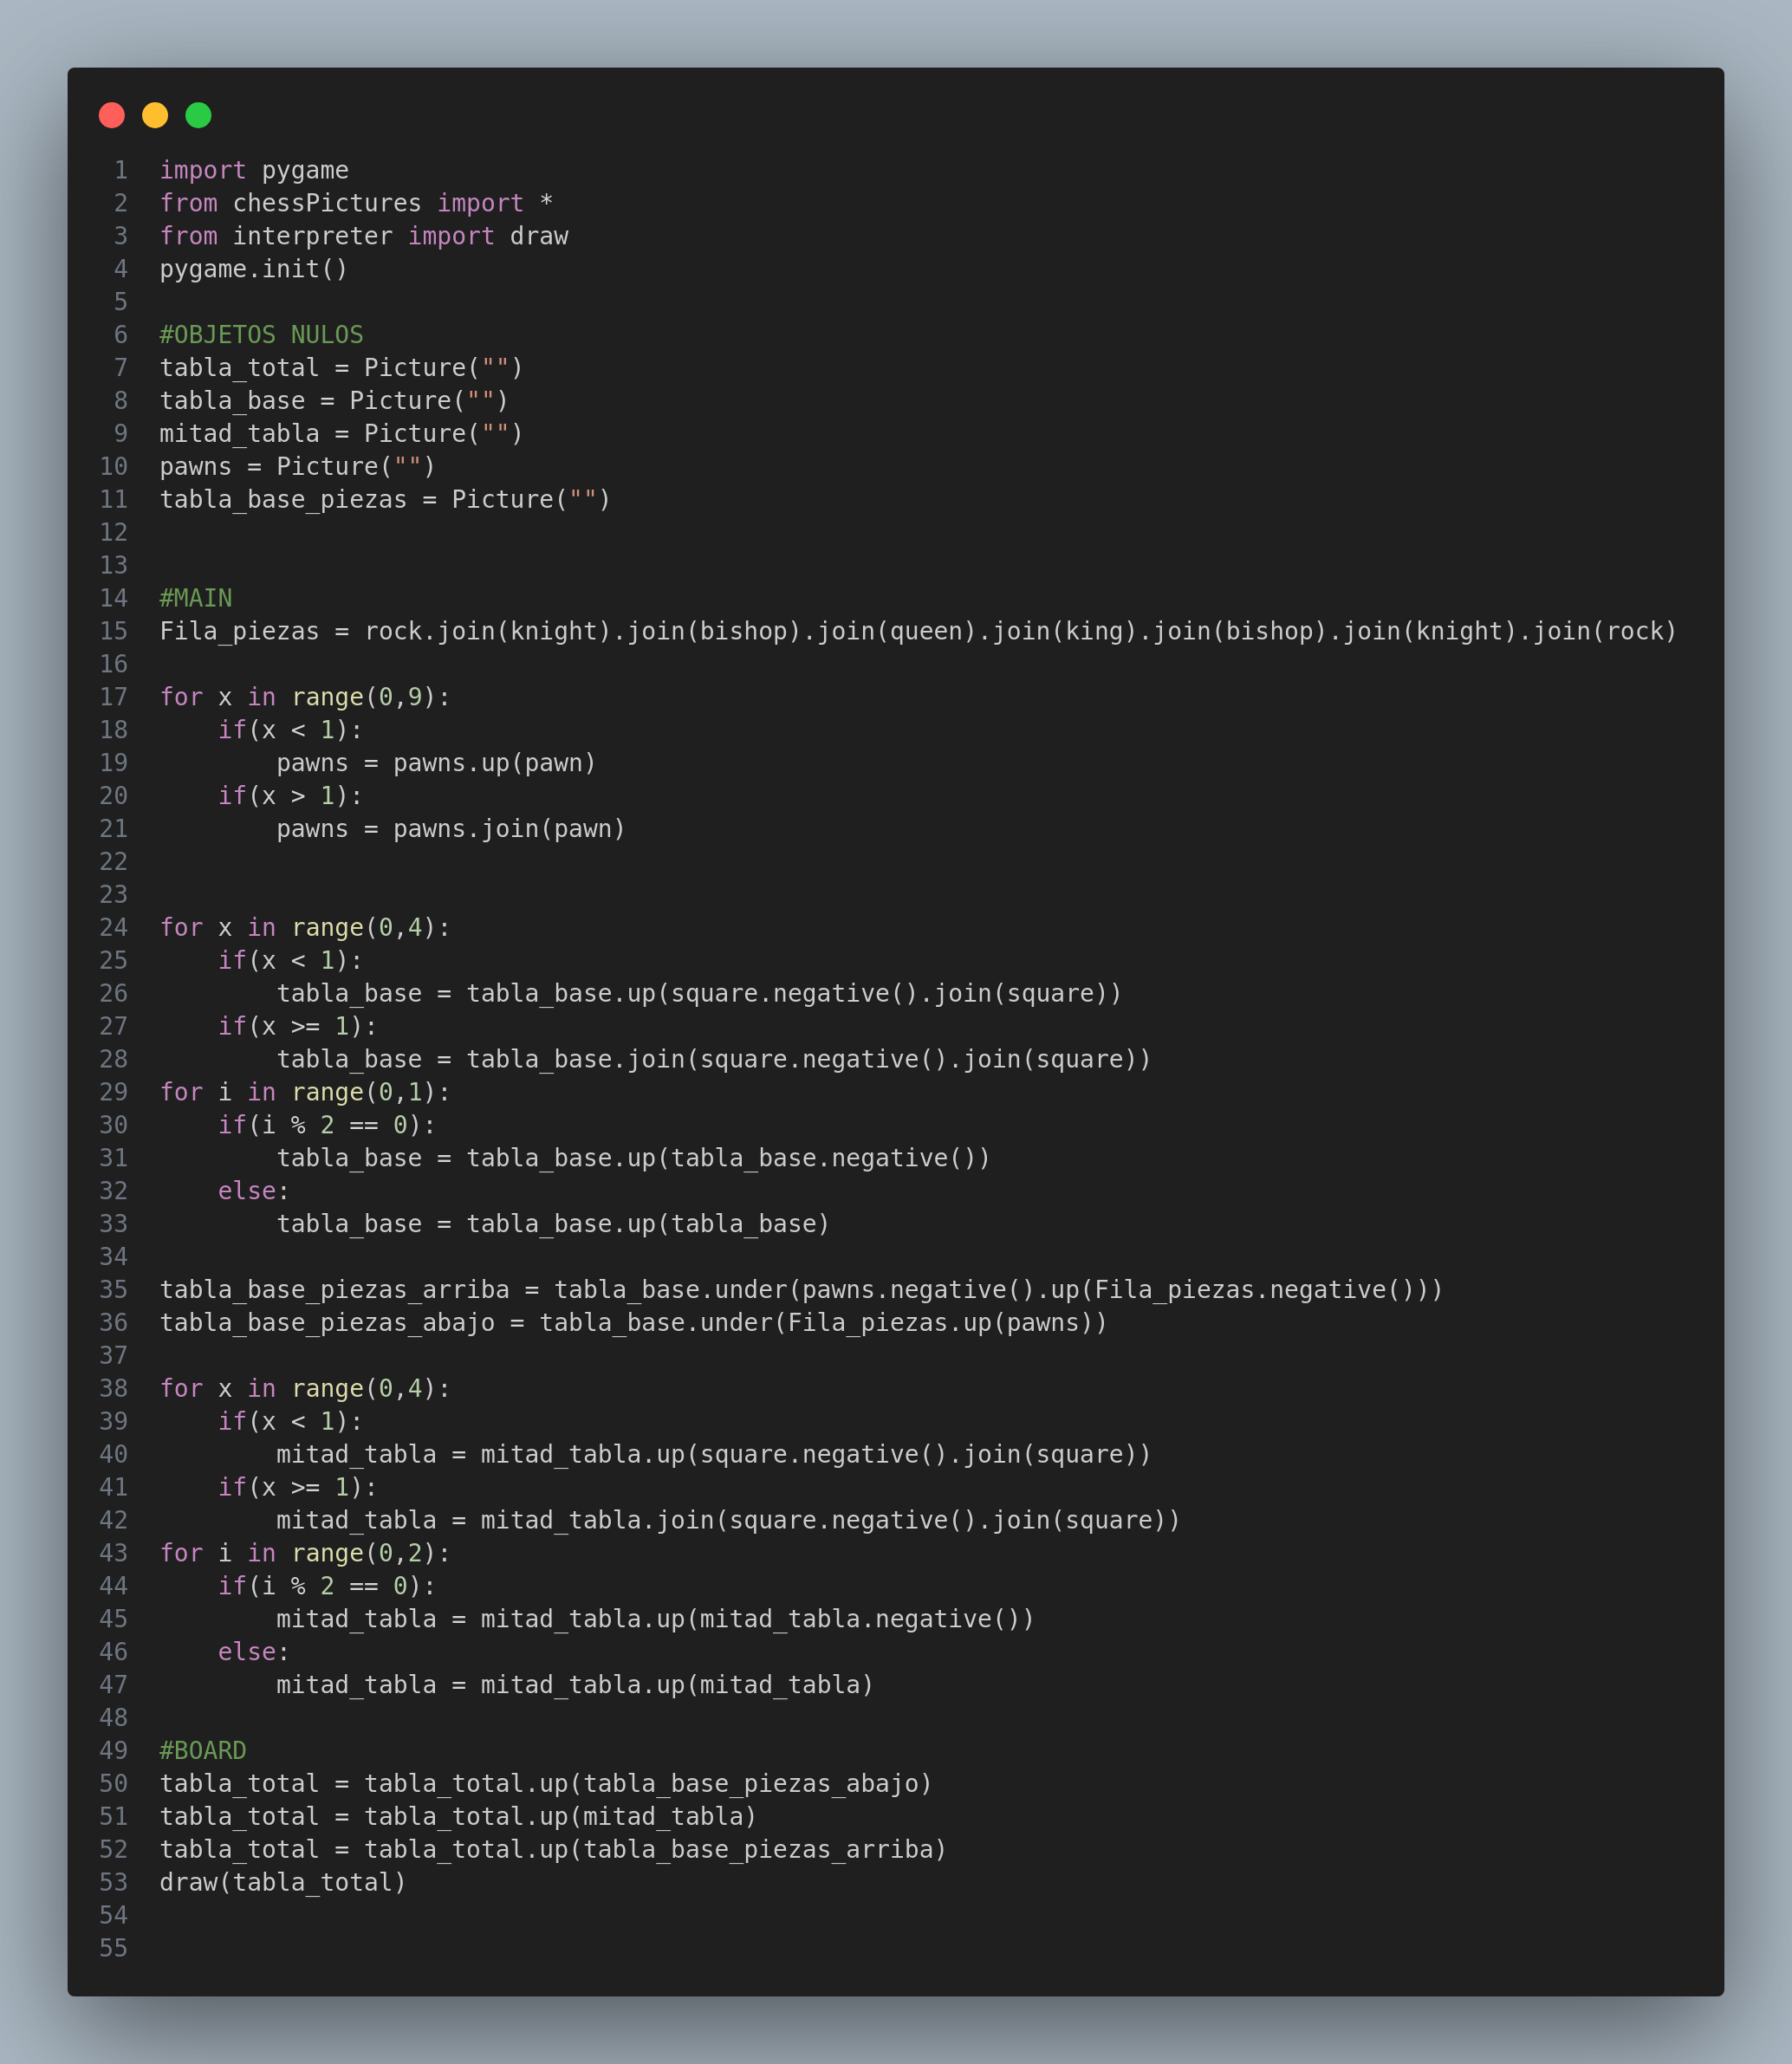
\includegraphics[width=0.7\textwidth]{img/Ej7.png}
  \caption{Codigo}
\end{figure}

\begin{figure}[H]
  \centering
  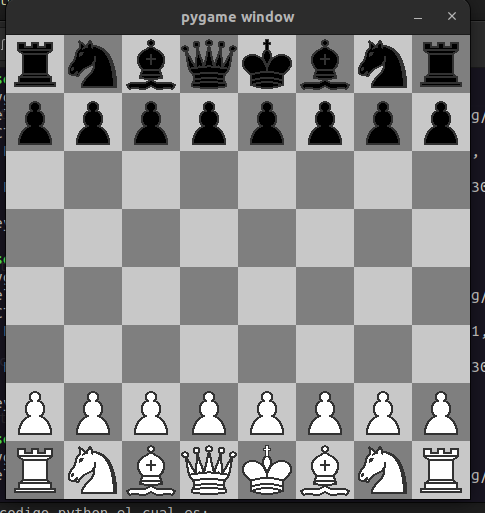
\includegraphics[width=0.7\textwidth]{img/Ejercicio7.png}
  \caption{Ejecucion}
\end{figure}

\section{Flip}
No carga mi video en flip por ellos use un link de drive
\begin{figure}[H]
  \centering
  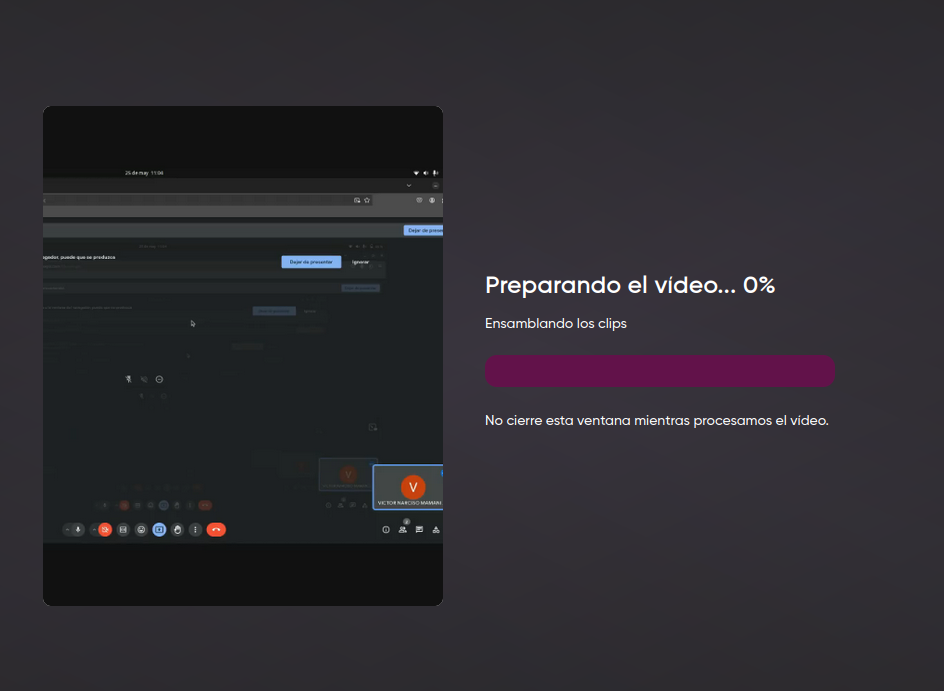
\includegraphics[width=0.7\textwidth]{img/Flip.png}
  \caption{Flip}
\end{figure}


\end{figure}
\item \textbf{URL de video de explicación:} \url{https://drive.google.com/file/d/1EeI8JwQNJr45i3DRMdqxW7Pbtwjt82PL/view}
\item \textbf{URL de repositorio de GitHub:} \url{https://github.com/VictorMA18/Lab05-Python}
\end{document}


